\chapter{What Is a Monster? Defining Yōkai}

\section{Why study monsters?}

The course starts from a simple claim: monsters are \emph{cultural artifacts}. They tell us
what a society fears, what it cannot explain, and where it draws its boundaries (between
human and animal, life and death, nature and culture, us and them). Japan is an especially
rich case because it has a continuous, well-documented monster tradition running from
eighth-century myth to Pokémon, and because that tradition has been consciously collected,
catalogued, illustrated and commercialized for at least three hundred years.

\begin{important}[Course questions]
\begin{enumerate}
  \item What \emph{is} a yōkai, and who decides?
  \item How do monsters change with media (oral legend, scroll, woodblock book, manga,
        film, game)?
  \item What work do monsters do for the people who imagine them (explaining, warning,
        entertaining, selling)?
  \item How did Japanese monsters become a global commodity?
\end{enumerate}
\end{important}

\section{Monster theory}

\subsection{Cohen's seven theses (1996)}

Jeffrey Jerome Cohen's essay ``Monster Culture (Seven Theses)'' is the starting point. In
my own paraphrase:

\begin{enumerate}
  \item The monster's body is a cultural body: it embodies a moment, a feeling, a place.
  \item The monster always escapes: it is killed but returns in new forms.
  \item The monster is a harbinger of category crisis: it refuses to fit (part animal, part
        human, dead but walking).
  \item The monster dwells at the gates of difference: the foreigner, the woman, the
        outsider are monstered.
  \item The monster polices the borders of the possible: do not go there, or this will
        happen to you.
  \item Fear of the monster is really a kind of desire: we are attracted to what we fear.
  \item The monster stands at the threshold of becoming: monsters ask us why we created
        them.
\end{enumerate}

\begin{example}[Category crisis]
The \emph{kappa} is reptile, amphibian, monkey and child at once; the \emph{nekomata} is a
cat that walks upright and speaks; the \emph{rokurokubi} is a woman whose neck stretches at
night. All are ``wrong'' combinations of familiar categories, which is precisely what makes
them unsettling (and, later, funny and cute).
\end{example}

\section{Defining yōkai}

\begin{definition}[Yōkai]
\emph{Yōkai} (\ja{妖怪}) is written with characters meaning ``bewitching/suspicious'' and
``strange/mysterious''. Following Michael Dylan Foster (\emph{Pandemonium and Parade},
2009; \emph{The Book of Yōkai}, 2015), the working definition is: a
\emph{weird or mysterious phenomenon, or the creature imagined to cause it}. Yōkai are
in-between: neither fully gods nor fully animals, neither clearly good nor clearly evil.
\end{definition}

\begin{remark}
The word \emph{yōkai} became the standard umbrella term only in the 20th century, largely
because of folklorists (Yanagita Kunio) and manga artist Mizuki Shigeru. Earlier periods
used many other words. Using ``yōkai'' for everything is therefore a slight anachronism,
but it is the convention of the field.
\end{remark}

\subsection{Related vocabulary}

\begin{center}
\begin{tabular}{lllp{6.5cm}}
\toprule
Term & Romaji & Literal & Usage \\
\midrule
\ja{妖怪} & yōkai & bewitching + strange & modern umbrella term \\
\ja{化け物} & bakemono & ``changed thing'' & shapeshifters; Edo-period common word \\
\ja{お化け} & obake & (polite) changed thing & childish/colloquial ``spook'' \\
\ja{物の怪} & mononoke & ``spirit of things'' & Heian possessing spirits (cf.\ Miyazaki's film) \\
\ja{幽霊} & yūrei & ``faint spirit'' & ghost of a dead human \\
\ja{怨霊} & onryō & ``resentful spirit'' & vengeful ghost (Week 4, Week 10) \\
\ja{鬼} & oni & ``demon/ogre'' & horned ogre, often of hell (Week 2) \\
\ja{怪獣} & kaijū & ``strange beast'' & giant monsters of film (Week 9) \\
\ja{妖精} & yōsei & ``bewitching spirit'' & modern word for Western fairies \\
\bottomrule
\end{tabular}
\end{center}

\subsection{Yōkai vs.\ yūrei}

\begin{center}
\begin{tabular}{p{3cm}p{5cm}p{5cm}}
\toprule
 & Yōkai \ja{妖怪} & Yūrei \ja{幽霊} \\
\midrule
Origin & animals, objects, places, nature & dead humans \\
Attachment & a place (bridge, river, mountain path) & a person (grudge, unfinished business) \\
Appearance & endlessly varied, often comic & standardized: white robe, long black hair, no feet \\
Time & dusk (\ja{逢魔時}, ōmagatoki, ``hour of meeting demons'') & ``hour of the ox'' (about 2 a.m.) \\
\bottomrule
\end{tabular}
\end{center}

\begin{aside}
Yanagita Kunio drew this distinction (yōkai haunt places, ghosts haunt people), but
students pointed out many exceptions (Oiwa haunts a person but appears in specific
places; the kitsune possesses people). The professor's answer: all categories in this
course are fuzzy, and that is the point.
\end{aside}

\section{A working taxonomy}

There is no official classification. The concept map below organizes the creatures that recur in the course by \emph{origin}.

\begin{center}
\begin{tikzpicture}[
    root/.style={draw, thick, rounded corners, fill=purple!20, font=\bfseries},
    cat/.style={draw, thick, rounded corners, fill=blue!10, font=\small, align=center, minimum width=2.3cm},
    ex/.style={font=\scriptsize, align=center}]
  \node[root] (y) at (0,0) {Japanese supernatural beings};
  \node[cat] (ani) at (-6,-2) {animal\\transformations};
  \node[cat] (hum) at (-3,-2) {human\\dead};
  \node[cat] (obj) at (0,-2) {objects\\(\ja{付喪神})};
  \node[cat] (nat) at (3,-2) {nature /\\places};
  \node[cat] (rel) at (6,-2) {religious\\figures};
  \foreach \c in {ani,hum,obj,nat,rel} \draw[->, thick] (y) -- (\c);
  \node[ex, below=0.2cm of ani] {kitsune \ja{狐}\\tanuki \ja{狸}\\bakeneko \ja{化け猫}};
  \node[ex, below=0.2cm of hum] {yūrei \ja{幽霊}\\onryō \ja{怨霊}\\ubume \ja{産女}};
  \node[ex, below=0.2cm of obj] {kasa-obake\\chōchin-obake\\bake-zōri};
  \node[ex, below=0.2cm of nat] {kappa \ja{河童}\\tengu \ja{天狗}\\yuki-onna \ja{雪女}};
  \node[ex, below=0.2cm of rel] {oni \ja{鬼}\\kami \ja{神}\\gaki \ja{餓鬼}};
\end{tikzpicture}
\end{center}

\begin{definition}[Tsukumogami]
\emph{Tsukumogami} (\ja{付喪神}) are household objects that come to life after about a
hundred years of use (or after being discarded): umbrellas, lanterns, sandals, tea
kettles. Medieval picture scrolls show them parading through the night; the idea reflects
both animism and anxiety about wasting things.
\end{definition}

\section{Kami, yōkai and the ``fallen god'' theory}

Yanagita Kunio proposed that yōkai are \emph{gods in decline}: kami who lost their worship
and became frightening or comic. The kappa, for example, may be a degraded water deity.

\begin{center}
\begin{tikzpicture}[b/.style={draw, thick, rounded corners, minimum width=2.6cm, align=center, font=\small}]
  \node[b, fill=yellow!25] (k) at (0,0) {kami \ja{神}\\(worshipped)};
  \node[b, fill=gray!20] (y) at (6,0) {yōkai \ja{妖怪}\\(not worshipped)};
  \draw[->, very thick] (k) to[bend left=20] node[above, font=\scriptsize] {loss of faith, neglect} (y);
  \draw[->, very thick] (y) to[bend left=20] node[below, font=\scriptsize] {enshrinement, festivals} (k);
\end{tikzpicture}
\end{center}

Komatsu Kazuhiko later revised this: the same being can be a kami when it is worshipped
and a yōkai when it is not, and movement goes \emph{both ways} (a vengeful spirit can be
pacified by being enshrined as a god, as with Sugawara no Michizane in Week 4).

\section{Media history of yōkai: a preview}

\begin{center}
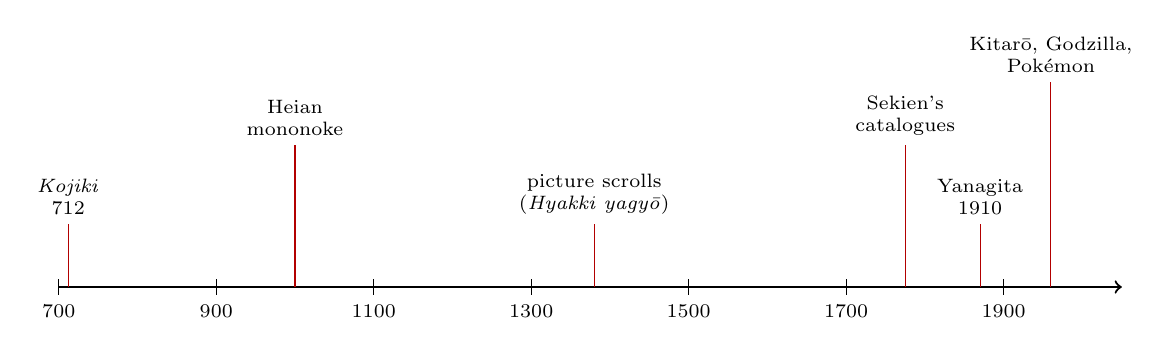
\begin{tikzpicture}[x=0.5cm, y=1cm, every node/.style={font=\scriptsize}]
  \draw[->, thick] (0,0) -- (27,0);
  \foreach \x/\l in {0/700, 4/900, 8/1100, 12/1300, 16/1500, 20/1700, 24/1900} {
    \draw (\x,0.1) -- (\x,-0.1) node[below] {\l};
  }
  \foreach \x/\h/\l in {0.24/0.8/{\emph{Kojiki}\\712}, 6/1.8/{Heian\\mononoke}, 13.6/0.8/{picture scrolls\\(\emph{Hyakki yagyō})},
      21.5/1.8/{Sekien's\\catalogues}, 23.4/0.8/{Yanagita\\1910}, 25.2/2.6/{Kitarō, Godzilla,\\Pokémon}} {
    \draw[red!70!black] (\x,0) -- (\x,\h);
    \node[above, align=center] at (\x,\h) {\l};
  }
\end{tikzpicture}
\end{center}

\section*{Summary}
\begin{itemize}
  \item Monsters are cultural artifacts that embody categories, fears and desires (Cohen).
  \item Yōkai: a mysterious phenomenon or the creature imagined to cause it (Foster);
        an in-between category.
  \item Know the vocabulary: yōkai, bakemono, obake, mononoke, yūrei, onryō, oni, kaijū.
  \item Yōkai vs.\ yūrei: place vs.\ person, varied vs.\ standardized.
  \item Kami and yōkai are two states of the same kind of being (Yanagita, Komatsu).
\end{itemize}
